%Pakete;
%A4, Report, 12pt
\documentclass[ngerman,a4paper,12pt]{scrreprt}
\usepackage[a4paper, right=20mm, left=20mm,top=20mm, bottom=30mm, marginparsep=5mm, marginparwidth=5mm, headheight=7mm, headsep=15mm,footskip=15mm]{geometry}

%Papierausrichtungen
\usepackage{pdflscape}
\usepackage{lscape}

%Deutsche Umlaute, Schriftart, Deutsche Bezeichnungen
\usepackage[utf8]{inputenc}
\usepackage[T1]{fontenc}
\usepackage[ngerman]{babel}

%quellcode
\usepackage{listings}

%tabellen
\usepackage{tabularx}

%listen und aufzählungen
\usepackage{paralist}

%farben
\usepackage[svgnames,table,hyperref]{xcolor}

%symbole
\usepackage{latexsym,textcomp}

%font
\usepackage{helvet}
\renewcommand{\familydefault}{\sfdefault}

%Abkürzungsverzeichnisse
\usepackage[printonlyused]{acronym}

%Bilder
\usepackage{graphicx} %Bilder
\usepackage{float}	  %"Floating" Objects, Bilder, Tabellen...
\usepackage[space]{grffile} %Leerzechen Problem bei includegraphics
\usepackage{wallpaper} %Seitenhintergrund setzen
\usepackage{transparent} %Transparenz

%for
\usepackage{forloop}
\usepackage{ifthen}

%Dokumenteigenschaften
\title{Repetitionsfragen CN1}
\author{Tobias Blaser}
\date{\today{}, Rapperswil}


%Kopf- /Fusszeile
\usepackage{fancyhdr}
\usepackage{lastpage}

\pagestyle{fancy}
	\fancyhf{} %alle Kopf- und Fußzeilenfelder bereinigen
	\renewcommand{\headrulewidth}{0pt} %obere Trennlinie
	\fancyfoot[L]{Seite \thepage/\pageref{LastPage}} %Fusszeile mitte
	\fancyfoot[R]{\today{}} %Fusszeile rechts
	\renewcommand{\footrulewidth}{0.4pt} %untere Trennlinie

%Kopf-/ Fusszeile auf chapter page
\fancypagestyle{plain} {
	\fancyhf{} %alle Kopf- und Fußzeilenfelder bereinigen
	\renewcommand{\headrulewidth}{0pt} %obere Trennlinie
	\fancyfoot[L]{Seite \thepage/\pageref{LastPage}} %Fusszeile mitte
	\fancyfoot[R]{\today{}} %Fusszeile rechts
	\renewcommand{\footrulewidth}{0.4pt} %untere Trennlinie
}

\usepackage{changepage}

%listen und aufzählungen
\usepackage{paralist}
\usepackage{mdwlist}

% list short cuts
\newcommand{\ul}{
	\begin{itemize}
}
\newcommand{\ulE}{
	\end{itemize}
}
\newcommand{\ol}{
	\begin{enumerate}
}
\newcommand{\olR}{
	\resume{enumerate}
}
\newcommand{\olE}{
	\end{enumerate}
}
\newcommand{\olS}{
	\suspend{enumerate}
}
\newcommand{\li}{
	\item
}
\newcommand{\dl}{
	\begin{description}
}
\newcommand{\di}[1]{
	\item[#1]
}
\newcommand{\dlE}{
	\end{description}
}
\newcommand{\ra}{
	$\rightarrow$
}

% chapter and section shortcuts
\newcommand{\ch}[1]{
	\chapter{#1}
}
\newcommand{\se}[1]{
	\section{#1}
}
\newcommand{\sse}[1]{
	\subsection{#1}
}
\newcommand{\sss}[1]{
	\subsubsection{#1}
}

%links, verlinktes Inhaltsverzeichnis, PDF Inhaltsverzeichnis
\usepackage[bookmarks=true,
bookmarksopen=true,
bookmarksnumbered=true,
breaklinks=true,
colorlinks=true,
linkcolor=black,
anchorcolor=black,
citecolor=black,
filecolor=black,
menucolor=black,
pagecolor=black,
urlcolor=black
]{hyperref} % Paket muss unbedingt als letzes eingebunden werden!

\usepackage{graphicx}
\begin{document}

% Inhaltsverzeichnis
\tableofcontents
\clearpage


\ch{Grundlagen}
\ol
	\li Abb. \ref{symb1} \& \ref{symb2}: Erklären Sie die folgenden Symbole: 
		\begin{figure}[H]
			\caption{}
			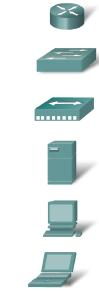
\includegraphics[scale=0.60]{img/R1.1.jpg}
			\label{symb1}
		\end{figure}
		\begin{figure}[H]
			\caption{}
			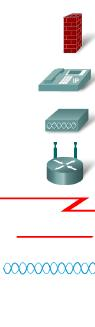
\includegraphics[scale=0.60]{img/R1.2.jpg}
			\label{symb2}
		\end{figure}			 
	\li Nennen Sie die Eigenschaften eines LAN.
	\li Was zeichnet ein WAN aus, welche Verbindungstopologien gibt es?
	\li Wie ist das Internet aufgebaut?
	\li Was Bedeuten Segmentation und Multiplexing in Bezug auf Netzwerkkommunikation?
	\li Was sind Intermedary Devices? Nennen Sie vier Gruppen mit konkreten Beispielen.
	\li Welche Aufgaben übernehmen Intermediary Devices? Nennen Sie mind. 4.
	\li Was ist ein Protokoll? Wie funktioniert es?
	\li Was ist ein Standard? Erklären Sie die Bedeutung von Standards in Netzwerkbereich.
	\li Erklären Sie das OSI Model. Nennen Sie zu jedem Layer die Aufgabe sowie Protokollbeispiele.
	\li Abb \ref{tcp}: Erklären Sie das folgende Bild:  	
		\begin{figure}[H]
			\centering
			\caption{}
			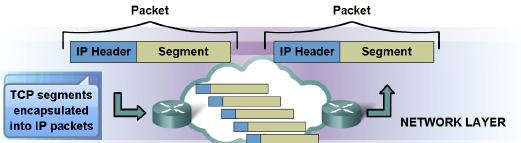
\includegraphics[scale=0.60]{img/R1.3.jpg}
			\label{tcp}
		\end{figure}	
	\li Abb \ref{signals}: Bennen Sie diese 3 Signale: 	
		\begin{figure}[H]
			\centering
			\caption{}
			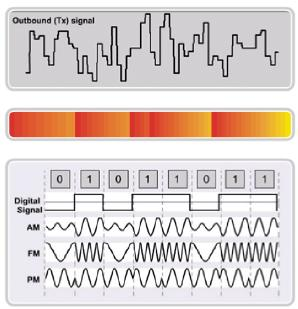
\includegraphics[scale=0.60]{img/R1.4.jpg}
			\label{signals}
		\end{figure} 
	\li Zeigen Sie Anhand eines Beispiels den Oberhead auf, der mit jedem Layer hinzukommt.
	\li Stellen Sie das TCP/IP Modell dem OSI Modell gegenüber.
\olS


\ch{Ethernet Grundlagen}
\olR
	\li Welche Aufgaben übernehmen die beiden Sublayer der OSI Schicht zwei?
	\li Erklären Sie den Unterschied zwischen Ethernet II und IEEE 802.3? Erklären Sie jeden Teil des Frames.
	\li Was ist ein Unicast? Was ein Multicast und was ein Broadcast?
	\li Wie ist die MAC Adresse aufgebaut? Was sind das Individual/Group Flag und was das Universal/Local Flag?
	\li Wie ist der LLC aufgebaut? Was sind DSAP und SSAP, was SNAP?
	\li Was ist Power-over Ethernet und wie funktioniert es?
	\li Wie funktioniert Energie effizientes Ethernet?
	\li Wie funktioniert die Frame Synchronisation beim Manchester Code?
	\li Wie hängen Kollisionsdetektion und Kollisionsfomäne zusammen beim Halb Duplex mode?
	\li Wie gross sind die die maximale Ausdehnungen der Kollisionsdomäne bei 10Base und 100 Base Ethernet? Was sind Late Collisions?
	\li Welchen Vorteil bietet Full Duplex Übertragung gegenüber Halb Duplex?
\olS


\ch{Fast \& Gigabit Ethernet}
\se{Fast Ethernet}
\olR
	\li Wie funktioniert die MLT-3 Codierung und warum werden dazu 4Bit mit 5Bit codiert? Was für eine effektive Übertragungsrate resultiert daraus beii einer 100Mbit/s Übertragung?
	\li Abb \ref{fasteth}: Welche Aufgaben Übernehmen GMII, PCS, PMA und PMD? Wie werden jeweils die Daten weitergereicht?
	 	\begin{figure}[H]
			\centering
			\caption{}
			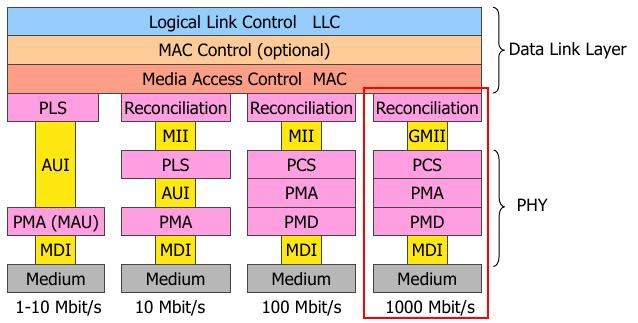
\includegraphics[scale=0.40]{img/R1.5.jpg}
			\label{fasteth}
		\end{figure}			 
	\li Aus welchem Grund werden bei Ethernet 1000Base-T alle 4 Adernpaare verwendet?
\olS
\se{Gigabit Ethernet}
\olR
	\li Aus welchem Grund erlaubt Gigabit Ethernet nur noch full-duplex mode und Kabel mit min. Cat6a?
	\li Abb \ref{gigabeth}: Welche Aufgaben übernehmen XGMII, 64Bit/66B PCS, WIS, PMA und PMD? Wie werden die Daten weitergereicht? 	
		\begin{figure}[H]
			\centering
			\caption{}
			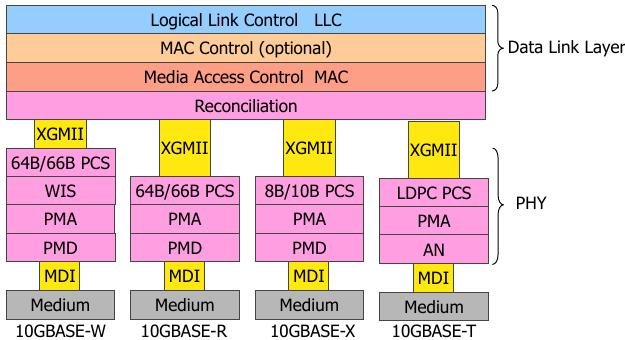
\includegraphics[scale=0.40]{img/R1.6.jpg}
			\label{gigabeth}
		\end{figure}			 
	\li Aus welchem Grund werden für lange Strecken vier parallele Glasfaserleitungen verwendet?
Wie werden die vier Datenströme auf kurzen Strecken in einer Faster transportiert?
\olS
\se{40/100 Gigabit Ethernet}
\olR
	\li Warum ist 40/100 Gigabit Ethernet nur über Glasfaserleitungen möglich, bzw. nur für ganz kurze Leitungen über Kupfer möglich?
\olS


\ch{LAN Design}
\se{Hardware}
\olR
	\li Nennen Sie 4 Aufgaben eines LAN.
	\li Wie funktionieren Repeater, Hub, Bridge, Switch und Router? Nennen Sie jeweils die Auswirkungen auf Collisions- und Broadcastdomain.
	\li Was kann ein Switch, was ein Hub nicht kann?
	\li Erklären Sie die vier "Forwarding Principles" die Switches umsetzen können.
	\li Was ist eine "Non Blocking Switching Fabric"?
	\li Welche beiden Architekturtypen gibt es bei Switches und welche Vor-/Nachteile besitzen sie?
\olS
\se{Spanning Tree Protokoll}
\olR
	\li Was kann in einem Redundanten Netzwerk ohne Spanning Tree passieren? warum? Wie löst das Spanning Tree Protocoll dieses Problem?
	\li Was ist die Bridge ID? Was sind Port Kosten?
	\li Wie wird die Rootbridge bestummen? WIe wird anschliessend weiter verfahren um den Spanning Tree zu bestimmen? Nach welchen Regeln wird vorgegangen?
	\li Abb \ref{stpex1}: Bestimmen Sie die Root Bridge und alle Pfade:
	\begin{figure}[H]
		\centering
		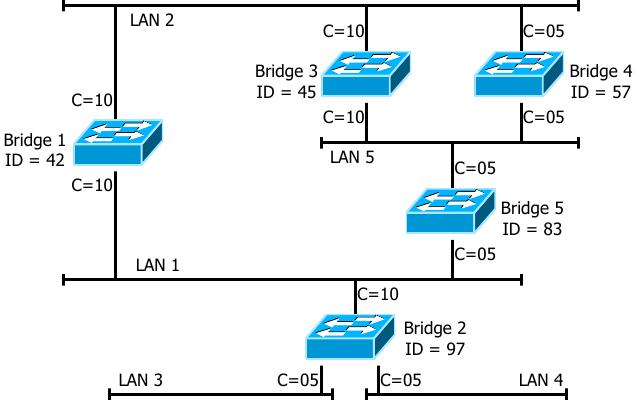
\includegraphics[scale=0.60]{img/R4.1.jpg}
		\caption{}
		\label{stpex1}
	\end{figure}
	\li Welche vier Stati können die Ports einnehmen? Was bedeuten Sie?
	\li Welche Vorteile bringt das RSTP gegenüber dem STP?
\olS


\ch{VLANs und Campus Design}
\se{VLANs}
\olR
	\li Nennen Sie einige Vorteile von VLANs.
	\li Was ist das sogenannte Tagging von Paketen bei VLANs? Wie ist es aufgebaut?
	\li Was ist eine Trunk Leitung?
	\li Wie wirken sich VLANs auf Broadcast- und Kollisionsdomäne aus?
	\li Warum braucht es zum Vermitteln zwischen VLANs Router? Warum kann dies kein Switch?
	\li Beschreiben Sie detailiert das Senden eines IP Paketes von einem Host in einem VLAN zu einem Host in einem andern VLAN.
	\li Was ist der Unterschied zwischen einem Router mit einem Trunkport und einem Router bei dem die verschiedenen VLANs über einzelne Ports angeschlossen werden?
	\li Was ist ein Layer 3 Switch? Was unterscheidet ihn von einem Router oder einem Switch?
	\li Welche drei Möglichkeiten gibt es, Stationen einem VLAN zuzuordnen?
	\li  Warum musste STP für VLANs erweitert werden? Welchen positiven Effekt haben VLANs auf die Ausnutzung redundanter Netze?
\olS

\se{Campus Design}
\olR
	\li Erklären Sie kurz, wie die folgenden Architekturen aufgebaut sind und nennen Sie die Vor- und Nachteile:
		\ol 
			\li Flaches Netzwerk
			\li Router-on-a-Stick Design
			\li Collapsed Backbone Design
			\li beide Arten von L3 Distribution Design
			\li Heutzutagige Multilayer Network Design
		\olE
	\li Was ist das Hot Standby Router Protocol?
	\li Was sind Phantom Router?
	\li Was sind die Unterschiede zum normalen Spanning Tree Design?
	\li Nennen Sie einige "Oversubscripten Guidelines" zum Netzwerkdesign.
	\li Warum sind Campus weite VLANs zu vermeiden?
	\li Macht es einen Unterschied, ob sie in einem Campus Backbone einen Switch oder einen Router einsetzen?
\olS


\ch{WLAN}
\olR
	\li Welche zwei Architekturen sind gemäss IEEE für WLAN vorgesehen?
	\li Was ist Extendes Service Set ESS? Wozu wird es verwendet und wie funktioniert es?
	\li Wie funktioniert die Centralized Intelligence Architektur? Wo liegen die Vorteile? Welche Nachteile gibt es?
	\li Welche Massnahmen punkto Power Management beinhaltet WLAN?
	\li Erklären Sie das "Carrier Sense Multiple Acces / Collision Avoidance" Paketmodell von WLAN. Welches sind die Hauptziele?
	\li Was ist das "Hidden Terminal" Problem, und wie wird es gelöst?
	\li Zeichnen Sie für CSMA/CA mit TX Reservation ein Framediagramm (nur schematisch), mit dem Sie die Funktion erläutern.
	\li Welche Frequenzbänder stehen für WLAN zur Verfügung? Welches Band bietet Welches Problem / andere Störgeräte?
	\li Was ist der DSSS Frequency Channel Plan? Warum können effektiv nur 3-4 Kanäle genutzt werden?
	\li Wie funktioniert "Dynamic Frequency Selection"?
	\li Der 802.11n Standard führt MIMO ein. Was ist es, und welche Vorteile ergeben sich daraus? Welche Nachteile haben sich durch den nun bewusst genutzten Effekt bei früherigen Standards ergeben?
	\li Was erwartet uns bei Gbps WLAN? Wie soll dies möglich sein?
	\li Wie stehen Datenrate und Reichweite miteinander in Verbindung? Welche Unterschiede bez. Reichweite gibt es zwischen 2.4 GHz und 5 GHz?
	\li Was ist "Effective Isotropic Radiated Power"? Welche Distanzen können Sie hier überbrücken? Was sagt der Gesetzgeber zur Sendeleistung?
	\li Welche Grundsätzlichen Schwachstellen ergeben sich durch ein Drahtlosnetzwerk?
	\li Wie sicher ist WEP? Was bietet WAP? Wovon ist bei WAP Person die Sicherheit direkt abhängig? Wie funktioniert WAP Enterprise? Wie wird verhindert, dass sich irgend jemand als Accespoint ausgeben kann?
	\li Abb. \ref{pegelplan} Erklären Sie den folgenden Pegelplan.
		\begin{figure}[H]
		\centering
		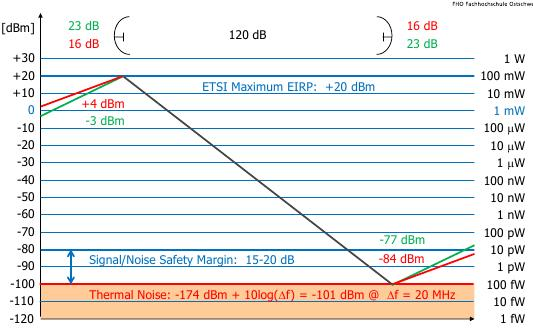
\includegraphics[width=\textwidth]{img/R6.1.jpg}
		\caption{}
		\label{pegelplan}
	\end{figure}
\olS


\ch{DSL}
\olR
	\li Was bedeuten DSL und DSLAM?
	\li Erklären Sie die Architektur einer DSL Verbindung vom Endgerät bis zum Provider.
	\li Wie wurde bei DSL nach und nach die Datenrate gesteigert? Welche Nachteile bringt dies mit sich?s
	\li Was bedeutet ``Fiber to the Curb''?
	\li Erklären Sie das ADSL/VDSL Kanalraster.
	\li Was sind POTS Spitter? Was ist das Guard Band?
	\li Warum stehen bei ADSL mit ISDN weniger Kanäle für Up- und Downstream zur Verfügung?
	\li Erklären Sie das DMT Verfahren.
	\li Erklären Sie die QAM Modulation.
	\li Was ist das Symbolsprektrum? Was ist OFDM?
	\li Wie berechnen Sie anhand der Symbolgrösser der einzelnen Kanäle die total mögliche Datenrate?
\olS


\ch{Internet Protocol}
\se{Grundlagen}
\olR
	\li Wie ist die Internet Society aufgebaut?
	\li Skizzieren Sie das OSI Model und benennen Sie die kleinste Nachrichteneinheit auf jeder Ebene.
	\li Skizzieren Sie den TCP/IP Protocol Stack. Wo liegen die Unterschiede zum OSI Model?
	\li Ordnen Sie die folgenden Begriffe den Layern des TCP/IP Protocol Stack zu:  POP, IMAP, FTP, Telnet, SSH, DNS, DHCP, TFTP, RARP, FDDI, ATM, X.25,ICMP, IPv4, IPv6,HTTP, SMTP,RTP, SIP,Ethernet, Token Ring, ARP, PPP,TCP, UDP
	\li Abb. \ref{LayNewoStr}: Erklären Sie die Grafik:
	\begin{figure}[H]
		\centering
		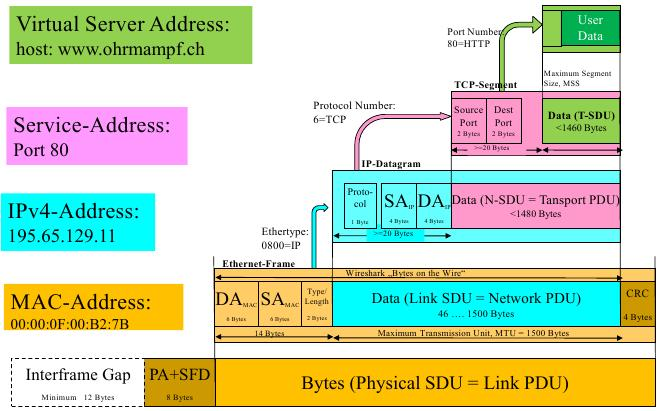
\includegraphics[width=\textwidth]{img/R8.1.jpg}
		\caption{}
		\label{LayNewoStr}
	\end{figure}
	\li 
	Wie funktioniert ein Netzerk Address Lookup? Machen Sie eine Skizze mit den Layern und dem entsprechenden Walk-trough.
	\li Erkären Sie, was ein Tier1 ISP, ein Tier2 ISP und ein Tier3 ISP ist.
	\li Was ist das "Autonomous System" AS? Welche drei Typen gibt es?
	\li Sie Senden einen Ping an www.google.ch. Skizzieren Sie den Weg des Pakets durch alle möglichen Hardwarekomponenten. Bauen Sie auch eine Firewall ein. Beschriften Sie alle Komponenten mit den Cisco Symbolen und deren Namen.
\olS

\se{IP}
\olR
	\li Erklären Sie die parallelen zwischen DNS und ARP.
	\li Wie ist eine IPv4 Adresse aufgebaut? Wie funktionieren Subnetmasken? 
	\li Berechnen Sie aus der IP Adresse 192.96.135.10/19 die IP Adresse binär und die Subnetmaske binär und in dezimaler Punkt schreibweise. In welchem Subnet befindet sich die IP Adresse? Wie lautet die Adresse der Station im Subnet? Welches ist die tiefste Adresse im Subnet, welche die höchste?
	\li Wie funktionieren Klassen basierte IP Adressen?
	\li Was sind "non-routable addresses"? Was steckt hinter den Adressen 10.0.0.0/8, 172.16.0.0/12 und 192.168.0.0/16?
	\li Wie viele non-routable Adressen kann man in einer Organisation maximal haben bei Class A, Class B, Class C und Total?
	\li Abb. \ref{netLayout}: Ein Paket wird von D nach E und eines von F nach B gesendet. Wie lauten auf jedem Abschnitt die Src.- und Dest.- MAC- und IP Adresse? Was passiert mit der Station C, die eine falsche Subnet Maske eingestellt hat? Wie lauten ihre Adresse im Subnet und das Subnet?
	\begin{figure}[H]
		\centering
		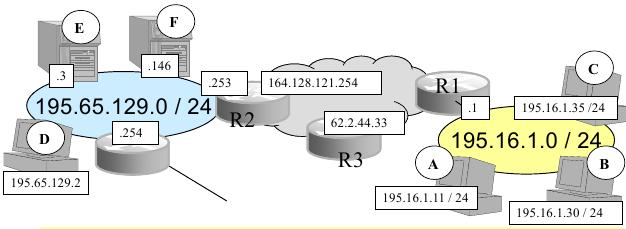
\includegraphics[width=\textwidth]{img/R9.1.jpg}
		\caption{}
		\label{netLayout}
	\end{figure}
	\li Wieso besitzen Router zwei IP Adressen?
	\li Abb. \ref{ipDatagram}: Erklären Sie jedes Kästchen der Grafik.
		\begin{figure}[H]
		\centering
		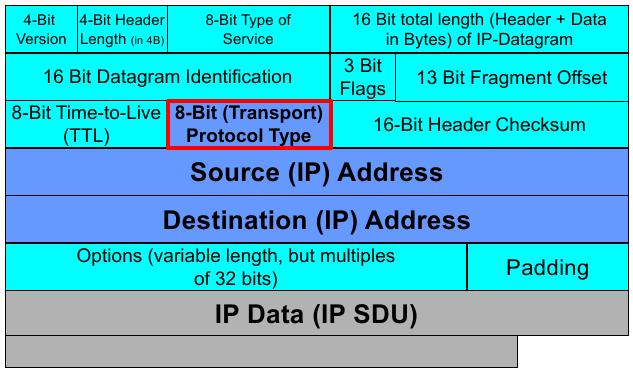
\includegraphics[width=\textwidth]{img/V9.4.jpg}
		\caption{}
		\label{ipDatagram}
	\end{figure}
	\li Was passiert, wenn die Time-to-live eines IP Paketes zu klein eingestellt ist?
	\li Warum können bei der Record Route nur maximal 9 Adressen aufgezeichnet werden? Was passiert, wenn es bis zum Ziel mehr Stationen sind, was wenn weniger?
	\li Wie funktioniert die fragmentation von Paketen? Wie wird der offset berechnet?
	\li Machen Sie eine Skizze: Fragmentieren Sie ein IP Datagram von 5140 Bytes für eine MTU von 1500 Bytes und geben Sie an, was jeweils im IP Header steht.
\olS

\se{Network Addess Translation}
\olR
	\li Was ist NAT? Was ist die NAT Tabble?
	\li Wozu dient NAT?
	\li Was ist PAT? Welche Unschönheiten ergeben sich dadurch? Welche Probleme kann es geben?
\olS


\ch{IPv6}
\olR
	\li Nennen Sie die entscheidentsten Veränderungen zwischen IPv4 und IPv6. Sprechen Sie insbesondere die folgenden Punkte an: Adresshirarchie, Datagram Fragmentation, ARP, IP Header, Security, Paket Identifikation.
	\li Erklären Sie folgende Adresstypen: Unicast, Multicast, Anycast.
	\li Wie ist eine IPv6 Adresse aufgebaut? Machen Sie eine Skizze.
	\li Wie setzt sich ie Interface ID ohne Privac Enhancement zusammen? Welche Vor- und Nachteile bringt dies mit sich?
	\li Was ist die Privacy Extension?
	\li Gegeben ist die folgende Adresse: 4501:6a8b::4:7bd:0:5e. Berechnen Sie die Adresse Binär. Geben Sie Registry (/23), Provider (/32), Subscriber (/48), Subnet (/64) und Interface ID in Hexadezimaler und Binärer Schreibweise an.
	\li Angenommen, die oben genannte Adresse wurde ohne Privacy Extension generiert. Wie lautet die zugehörige MAC Adresse der Schnittstelle?
	\li (Opt.) Für jedes wievielte Atom im Universum können Sie eine IPv6 Adresse vergeben?
	\li Welche Bedeutung kommt folgenden Adressen zu:
		\ol
			\li fe80::/10
			\li fec0::/10
			\li 2000::/3
			\li 2001::/32
			\li 2002::/16
			\li FF08
		\olE
	\li Wie ist der IPv6 Header aufgebaut? Machen Sie eine Skizze. Machen Sie auch eine Skizze für den IPv4 Header und zeichnen Sie die Unterschiede und die Gemeinsamkeiten ein.
	\li Welche drei Technologien werden für den Übergang von IPv4 zu IPv6 verwendet?
	\li Was bedeutet Dual-Stack Betrieb?
	\li Machen Sie eine Skizze von einem IPv6 Paket getunnelt in einem IPv4 Paket und umgekehrt.
	\li Welche vier Tunneling Prinzipien gibt es?
\olS


\ch{ICMP}
\olR
	\li Was bedeutet Ping?
	\li Welche Aufgaben übernimmt ICMP?
	\li Wie können Sie mit Ping die Verbindungsgeschwindigkeit in etwa ermitteln?
	\li Welche Probleme gibt es bei PAT und ICMP? Wie wird das umgangen?
\olS


\ch{Transport Layer Protokolle}
\olR
	\li Was ist ein Socket? Wie unterscheiden sich TCP- und UDP Socket?
	\li Was bedeutet "logischer End-zu-End" transport?
	\li Welche drei Typen von Port Nummern gibt es?
\olS

\se{UDP}
\olR
	\li Wie ist UDP aufgebaut? Machen Sie eine SKizze.
	\li Nennen Sie zwei zentrale Eigenschaften von UDP, die es von TCP unterscheiden.
	\li Folgender Hex Dump eines UDP Pakets ist bekannt: \\00 00 C0 23 AA A8 00 10 5A 22 12 C4 08 00 45 00
 00 1D 02 06 00 00 80 11 17 D1 98 60 78 16 98 60
 78 22 0F A0 0F A1 00 09 BE A1 01 00 00 00 00 00
 00 00 00 00 00 00 00 00 00 00 00 00 (a byte UDP-Data)
 		\ol
 			\li Zeichnen Sie das IP und das UDP Paket ein.
 			\li Geben Sie Source- und Destination Port sowie UDP Length an.
 			\li Welcher Wert steht im IP Header als Protokoll?
 		\olE
	 \li Warum besitzt UDP auch eine Checksumme?
	 \li Was müssen Sie beim UDP Demutliplexing unternehmen, damit Sie als Server die einzelnen Clients unterscheiden können? Machen Sie eine entsprechende Skizze mit einem Server und zwei Clients. Zeichnen Sie die Datenflüsse ein und schreiben Sie alle Port-Nummern an.
\olS






\end{document}
